\documentclass[11pt, xcolor={dvipsnames}, hyperref={colorlinks, allcolors=Blue}]{beamer}


% Packages
\usepackage{graphicx}
\usepackage{caption, subcaption}
\usepackage{tikz}
\usepackage{amsmath, amsfonts, amssymb}
\usepackage{bm}
\usepackage{booktabs}
\usepackage{apacite}
\usepackage{multirow}
\usepackage{multicol}
\usepackage{doi}
\usepackage{textpos}
\usepackage{lipsum}
\usepackage{amsfonts, amsmath}
\usepackage{wrapfig}
\usepackage{animate}
\usepackage{cleveref}


\renewcommand\doiprefix{}


\usepackage{tikz}
\usetikzlibrary{shapes, fit}





%%%%%%%%%%%%%%%%%%%%%%%%%%%%%%%%%%%%%%%%%%%%%%
% Custom commands
\newcommand\bc[1]{{\usebeamercolor[fg]{frametitle} {\textbf{#1}}}} % bold and color
\newcommand{\into}{\rightarrow}



%%%%%%%%%%%%%%%%%%%%%%%%%%%%%%%%%%%%%%%%%%%%%%
% Set Theme
\usetheme{Boadilla}
\usecolortheme{rose}

%%%%%%%%%%%%%%%%%%%%%%%%%%%%%%%%%%%%%%%%%%%%%%
% Make citation font tiny
\renewcommand{\bibliographytypesize}{\tiny}

%%%%%%%%%%%%%%%%%%%%%%%%%%%%%%%%%%%%%%%%%%%%%%
% Fonts
\usefonttheme{serif} % Serif font
\setbeamertemplate{enumerate items}[default] % Don't use bullets in enumerate.

%%%%%%%%%%%%%%%%%%%%%%%%%%%%%%%%%%%%%%%%%%%%%%%
% Remove navigation bar
\setbeamertemplate{navigation symbols}{}
%%%%%%%%%%%%%%%%%%%%%%%%%%%%%%%%%%%%%%%%%%%%%%


% Frontmatter
\title[ECON 8000 -  Lecture 8]{Lecture 8: Optimization}
\author[University of Queensland]{Robert Garrard}
\date[\today]{} 


%%%%%%%%%%%%%%%%%%%%%%%%%%%%%%%

% Common commands

% Sets
\newcommand{\R}{\mathbb{R}}
\newcommand{\N}{\mathbb{N}}
\newcommand{\Z}{\mathbb{Z}}
\newcommand{\Q}{\mathbb{Q}}
\renewcommand{\P}{\mathbb{P}}
\newcommand{\E}{\mathbb{E}}

% Symbols
\renewcommand{\epsilon}{\varepsilon}
\renewcommand{\implies}{\Rightarrow}
\newcommand{\halmos}{\hfill$\blacksquare$}

% Vector notation
\renewcommand{\a}{\mathbf{a}}
\renewcommand{\b}{\mathbf{b}}
\newcommand{\h}{\mathbf{h}}
\newcommand{\x}{\mathbf{x}}
\newcommand{\X}{\mathbf{X}}
\newcommand{\y}{\mathbf{y}}
\newcommand{\z}{\mathbf{z}}
\renewcommand{\v}{\mathbf{v}}
\newcommand{\bepsilon}{\mathbf{\varepsilon}}
\newcommand{\bbeta}{\mathbf{\beta}}

% Matrices
\newcommand{\eyetwo}{\begin{pmatrix} 1 & 0\\ 0 & 1 \\ \end{pmatrix}} % I_2 identity matrix
\newcommand{\eyethree}{\begin{pmatrix} 1 & 0 & 0\\ 0 & 1 & 0\\ 0 & 0 & 1 \end{pmatrix}} % I_3 identity matrix
\newcommand{\zerotwo}{\begin{pmatrix} 0 & 0\\ 0 & 0 \\ \end{pmatrix}} % 2x2 Zero matrix
\newcommand{\zerothree}{\begin{pmatrix} 0 & 0 & 0\\ 0 & 0 & 0\\ 0 & 0 & 0 \end{pmatrix}} % 3x3 Zero matrix


% Misc

\newcommand{\innerprod}[2]{\langle #1, #2 \rangle}


%%%%%%%%%%%%%%%%%%%%%%%%%%%%%%%%

% Tikz
\usetikzlibrary{arrows,shapes,trees, positioning}

%%%%%%%%%%%%%%%%%%%%%%%%%%%%%%

\newcounter{Lecture}
\addtocounter{Lecture}{8}

\newcounter{exercise}
\newenvironment{exercise}[1][]{\refstepcounter{exercise}\par\medskip
   \noindent {\bc{Exercise}~\bc{\theLecture.\theexercise} #1}}{\medskip}


\begin{document}

\begin{frame}
\titlepage

%\begin{picture}(0,0)
%\put(35,-50){\hbox{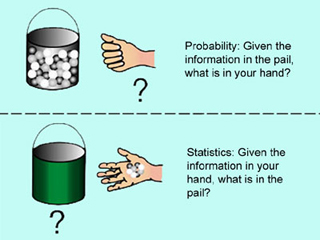
\includegraphics[width=0.8\textwidth, trim={0cm, 1cm, 0cm, 1cm}, clip]{prob_stats}}}
%\end{picture}

\end{frame}

%%%%%%%%%%%%%%%%%%%%%%%%%%%%%%%%%%%%%%%%%%%%%%%%%%%%%%%%

\begin{frame}{The Unconstrained Maximization Problem}

Let $X \subset \R^{n}$ and $f:X \into \R$. 
\bigskip

The \bc{interior} of a set $X$ is the set

\[ int\left(X\right) = \{\x \in X \ | \ \exists r > 0 \ s.t \ B(\x, r) \subset X\}\]

\bigskip
Consider the following maximisation problem
\large
\[ \underset{\x\in int\left(X\right)}{\mathrm{max}} \quad f(\x) \]
\normalsize

\end{frame}

\begin{frame}{The Unconstrained Maximization Problem}
The solution to this problem is the set

\[ S = \{ \x \in int\left(X\right) \ | \ f(\x) \geq f(\a) \ \ \forall \a \in int\left(X\right) \} \]
\bigskip

The fact that we're doing this over the interior of the set makes the problem \bc{unconstrained}.
\bigskip

 If we were to allow for maximisers to come from the boundary of the set, then the problem would be \bc{constrained} by the boundary. 
\vfill\vfill
\end{frame}
%%%%%%%%%%%%%%%%%%%%%%%%%%%%%%%%%%%%%%%%%%%%%%%%%%%%%%%%
\begin{frame}{First Order Condition}


\begin{block}{Proposition}
Let $f:X\into R$ be a $\mathcal{C}^{1}$ function defined on a subset of $\R^{n}$. If $\x_{0}$ is a local maximum (or minimum) of $f$ and $\x_{0} \in int\left(X\right)$, then

\[ \nabla f(\x_{0}) = 0\]
\end{block}

\bigskip
The proof for this is identical to the one variable case. 

\vfill\vfill
\end{frame}

%%%%%%%%%%%%%%%%%%%%%%%%%%%%%%%%%%%%%%%%%%%%%%%%%%%%%%%%
\begin{frame}{Second Order Condition}

\begin{block}{Proposition}
Let $f:X\into\R$ be a $\mathcal{C}^{2}$ function defined on a subset of $\R^{n}$. Suppose that $\x_{0}$ is a critical point of $f$. 

\begin{itemize}
\item[] If $D^{2}f(\x_{0})$ is \bc{negative definite}, then $\x_{0}$ is a local maximum
\item[] If $D^{2}f(\x_{0})$, is \bc{positive definite}, then $\x_{0}$ is a local minimum
\item[] If $D^{2}f(\x_{0})$, is \bc{indefinite}, then $\x_{0}$ is neither a max or a min
\end{itemize}
\end{block}
\vfill\vfill
\end{frame}

%%%%%%%%%%%%%%%%%%%%%%%%%%%%%%%%%%%%%%%%%%%%%%%%%%%%%%%%
\begin{frame}{The Unconstrained Optimization Recipe}

\begin{enumerate}[1.]
\setlength\itemsep{3mm}
\item Find the partial derivatives with respect to each of your choice variables. Set them equal to zero. Solve the system of equations for the set of critical points.

\item Check the definiteness of the Hessian at each of these critical points. Discard any points which do not meet the necessary conditions for a maximum. 

\item Plug each remaining critical point into the objective function a check which gives the highest value. 

\item Consider the behaviour of the objective function near the boundary. Remember, there may not even be a solution!

\end{enumerate}

\end{frame}

%%%%%%%%%%%%%%%%%%%%%%%%%%%%%%%%%%%%%%%%%%%%%%%%%%%%%%%%
\begin{frame}{Concavity and Convexity}
\begin{theorem}
Let $f:X\into\R$ be a $\mathcal{C}^{2}$ function whose domain is a convex open subset of $\R^{n}$.

\begin{enumerate}[a)]
\item The following conditions are equivalent
\begin{enumerate}[i)]
\item $f$ is a concave function on $X$
\item $f(\y) - f(\x) \leq Df(\x)\left (\y - \x \right ) \quad \forall \x,\y \in X$
\item $D^{2}f(\x)$ is negative semidefinite for all $\x \in X$
\end{enumerate}

\item The following conditions are equivalent
\begin{enumerate}[i)]
\item $f$ is a convex function on $X$
\item $f(\y) - f(\x) \geq Df(\x)\left (\y - \x \right ) \quad \forall \x,\y \in X$
\item $D^{2}f(\x)$ is positive semidefinite for all $\x \in X$
\end{enumerate}

\item If $f$ is a concave function on $X$ and $Df(\x^{*}) = 0$ for some $\x^{*} \in X$, then $\x^{*}$ is a global max of $f$ on $X$

\item If $f$ is a convex function on $X$ and $Df(\x^{*}) = 0$ for some $\x^{*} \in X$, then $\x^{*}$ is a global min of $f$ on $X$

\end{enumerate}

\end{theorem}
\end{frame}

%%%%%%%%%%%%%%%%%%%%%%%%%%%%%%%%%%%%%%%%%%%%%%%%%%%%%%%%
\begin{frame}{Exercises}
\begin{exercise}
For the following functions, find the critical points and classify these as local max, local min, saddle points, or ``can't tell''.
\begin{enumerate}[a)]
	\item $x^{4} + x^{2} - 6xy + 3y^{2}$
	\item $xy^{2} + x^{3}y - xy$
\end{enumerate}
\end{exercise}
\vfill\vfill 
\end{frame}
%%%%%%%%%%%%%%%%%%%%%%%%%%%%%%%%%%%%%%%%%%%%%%%%%%%%%%%%


\begin{frame}{Exercises}

\begin{exercise}


A perfectly competitive firm produces a final consumption good using labour and capital inputs. Labour is paid a wage $w$ and capital is rented at a rate $r$. The firm faces a constant returns to scale Cobb-Douglas production technology. All capital is returned after production. The price of the final good is normalised to 1. How does the firm choose labour and capital input so as to maximise profit?\\

Solve the firm's problem:

\[ \underset{\{L,K\}}{\mathrm{max}} \quad K^{\alpha}L^{1-\alpha} - wL - rK \]

\end{exercise}

\end{frame}


%%%%%%%%%%%%%%%%%%%%%%%%%%%%%%%%%%%%%%%%%%%%%%%%%%%%%%%%
\begin{frame}{Equality Constrained Optimization}
Consider the optimisation problem

\begin{align*}
\underset{\{x_{1}, x_{2}\}}{\mathrm{max}}  \quad& f(x_{1}, x_{2})\\
\text{s.t}\quad \ \ & g(x_{1}, x_{2}) = h
\end{align*}

To determine what conditions might be necessary for an optimum, consider these functions and their level sets.

\begin{figure}
	\begin{subfigure}[b]{0.45\textwidth}
		\centering
		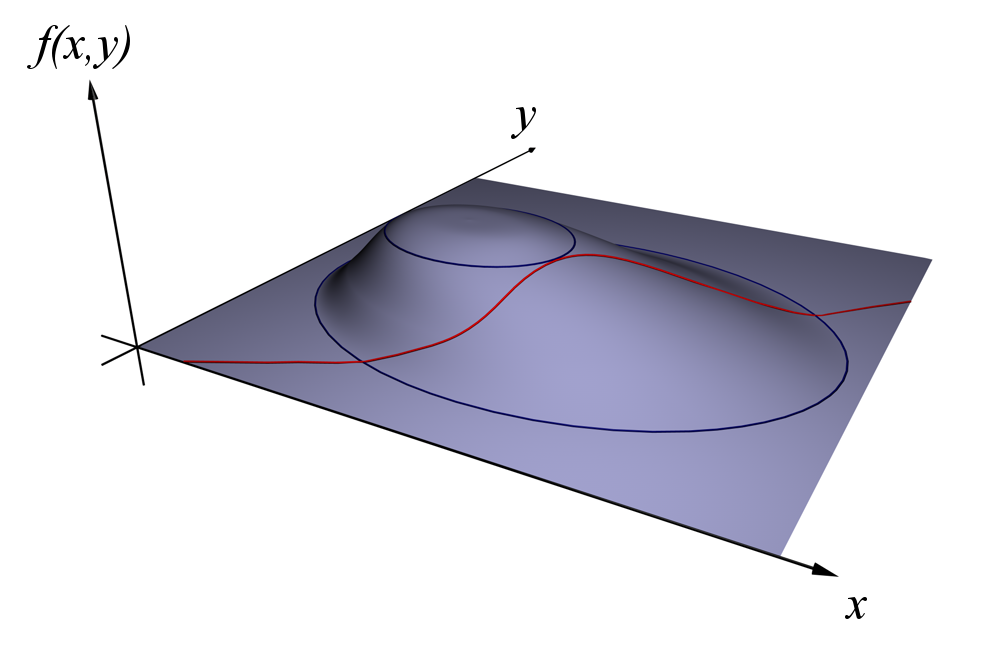
\includegraphics[width=\textwidth]{LagrangeMultipliers3D.png} 
	\end{subfigure}\hfill
	\begin{subfigure}[b]{0.45\textwidth}
		\centering
		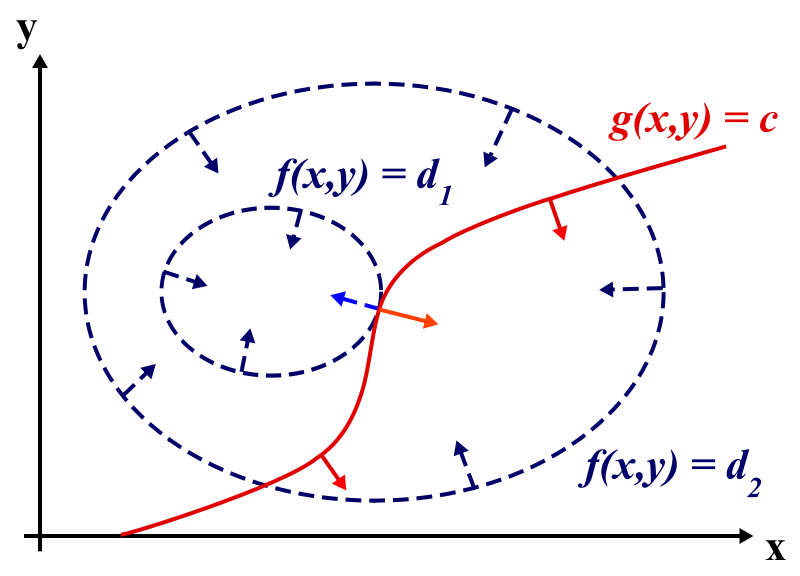
\includegraphics[width=\textwidth]{LagrangeMultipliers2D.png} 
	\end{subfigure}\hfill
\end{figure}


\end{frame}


%%%%%%%%%%%%%%%%%%%%%%%%%%%%%%%%%%%%%%%%%%%%%%%%%%%%%%%%
\begin{frame}{Equality Constrained Optimization}
If the level set of the objective function and the constraint set aren't tangential at some point, then they cross. \bigskip

This means we could move along the constraint set while at the same time moving up to a higher level curve (and so a higher value for the objective function). \bigskip

It must be the case then that at an optimum, the level set of the function and the constraint set are tangential. \\


\[\nabla f(\x^{*}) = \lambda \nabla g(\x^{*})\]
\smallskip

This is true whether we are maximising or minimising the objective.
\vfill\vfill

However, for $\lambda$ to be uniquely defined, we need to require that $\nabla g(\x^{*}) \not = 0$.

\end{frame}

%%%%%%%%%%%%%%%%%%%%%%%%%%%%%%%%%%%%%%%%%%%%%%%%%%%%%%%%
\begin{frame}{Equality Constrained Optimization}
Now consider the optimisation problem with several binding constraints

\begin{align*}
\underset{\{x_{1}, x_{2}\}}{\mathrm{max}}  \quad& f(x_{1}, x_{2},\dots, x_{n})\\
\text{s.t}\quad \ \ & g_{1}(x_{1}, x_{2},\dots,x_{n}) = h_{1}\\
\text{s.t}\quad \ \ & g_{2}(x_{1}, x_{2},\dots,x_{n}) = h_{2}\\
& \vdots\\
\text{s.t}\quad \ \ & g_{m}(x_{1}, x_{2},\dots,x_{n}) = h_{m}\\
\end{align*}


At the optimum, $\x^{*}$, it's still necessary that each of the constraint sets are tangential to the level curve of the objective function. \bigskip

We still need $\x^{*}$ not to be a critical point of \emph{any} of the constraint functions.


\end{frame}

%%%%%%%%%%%%%%%%%%%%%%%%%%%%%%%%%%%%%%%%%%%%%%%%%%%%%%%%
\begin{frame}{Non-degenerate Constraint Qualification}
Consider the Jacobian matrix of the constraint functions at $x^{*}$
\bigskip

\large
\[
\renewcommand{\arraystretch}{1.3}
D\h(\x^{*}) = 
\begin{pmatrix}
\frac{\partial h_{1}}{\partial x_{1}}  &  \dots &  \frac{\partial h_{1}}{\partial x_{n}}\\
\frac{\partial h_{2}}{\partial x_{1}} & \dots & \frac{\partial h_{2}}{\partial x_{n}}\\
\vdots & \ddots & \vdots\\
\frac{\partial h_{m}}{\partial x_{1}} & \dots & \frac{\partial h_{m}}{\partial x_{n}}\\
\end{pmatrix}
\]
\normalsize
\bigskip

The largest the rank of this Jacobian can be is $m$ (since we assume to have $m < n$). Not having $x^{*}$ be a critical point of any constraint is equivalent to saying that this Jacobian has full rank. This is known as the \bc{Non-degenerate Constraint Qualification} (NDCQ).\bigskip

Linear constraints always satisfy the NDCQ.

\end{frame}

%%%%%%%%%%%%%%%%%%%%%%%%%%%%%%%%%%%%%%%%%%%%%%%%%%%%%%%%
\begin{frame}{The Theorem of Lagrange}

\begin{theorem}
Let $f:\R^{n}\into \R$ be a $\mathcal{C}^{1}$ function. Consider the problem of maximising (or minimising) $f$ on the constraint set
\[C_{h} = \{\x \in \R^{n} \ | \ h_{i}(\x) = a_{i} \  \forall i = 1,2,\dots,m\}\]

Suppose that $\x^{*} \in C_{h}$ is a local max or min of $f$ on $C_{h}$ and $x^{*}$ satisfies the NDCQ. \\

Then there exist $\lambda^{*} = (\lambda_{1}^{*},\dots, \lambda_{n}^{*})$ such that $(\x^{*}, \lambda^{*})$ is a critical point of the Lagrangian
\[ \mathcal{L} = f(\x) + \lambda_{1} \left [ a_{1} - h_{1}(\x)\right] + \dots + \lambda_{n} \left [ a_{n} - h_{n}(\x)\right] \]
\end{theorem}


\end{frame}

%%%%%%%%%%%%%%%%%%%%%%%%%%%%%%%%%%%%%%%%%%%%%%%%%%%%%%%%
\begin{frame}{The Theorem of Lagrange}
\begin{block}{Example}
A consumer has a budget of $w$ dollars which they can spend on a mixture of consumption goods, $c_{1}$ and $c_{2}$; costing $p_{1}$ and $p_{2}$ dollars respectively. Their preferences are represented by $U(c_{1}, c_{2}) = c_{1}^{\alpha}c_{2}^{\beta}$, $\alpha + \beta \leq 1$. Set up and solve the consumer's utility maximization problem. \bigskip

\begin{gather*}
\underset{\{c_{1}, c_{2}\}}{\max} \ c_{1}^{\alpha}c_{2}^{\beta}\\
\text{s.t. } \quad p_{1}c_{1} + p_{2}c_{2} = w
\end{gather*}

which yields the lagrangian

\[\mathcal{L} = c_{1}^{\alpha}c_{2}^{\beta} + \lambda\left[w -p_{1}c_{1} - p_{2}c_{2} \right] \]

\end{block}
\end{frame}

\begin{frame}{The Theorem of Lagrange}
\begin{block}{Example}
Setting $\nabla \mathcal{L} = 0$ yields the first order conditions:

\begin{align}
\alpha c_{1}^{\alpha - 1}c_{2}^{\beta} - \lambda p_{1} = 0\\
\beta c_{1}^{\alpha }c_{2}^{\beta-1} - \lambda p_{2} = 0\\
p_{1}c_{1} + p_{2}c_{2} = w
\end{align}

Dividing (1) and (2) gives 
\[\frac{\alpha c_{2}}{\beta c_{1}} = \frac{p_{1}}{p_{2}} \implies c_{2} = \frac{\beta p_{1}}{\alpha p_{2}} c_{1}\]

Subbing into (3) gives

\[ p_{1}c_{1} = \frac{\alpha}{\alpha + \beta} w \qquad p_{2}c_{2}= \frac{\beta}{\alpha + \beta} w\] 

\end{block}
\end{frame}

%%%%%%%%%%%%%%%%%%%%%%%%%%%%%%%%%%%%%%%%%%%%%%%%%%%%%
\begin{frame}{Exercises}
\begin{exercise}

\begin{gather*}
\underset{\{x, y\}}{\max} \quad x \\
\text{s.t.} \quad x^{3} + y^{2} = 0
\end{gather*}
\end{exercise}
\vfill\vfill
\bigskip\vfill\vfill
\end{frame}

%%%%%%%%%%%%%%%%%%%%%%%%%%%%%%%%%%%%%%%%%%%%%%%%%%%%%
\begin{frame}{Second Order Conditions}

Second order conditions are substantially more difficult to check in the constrained case. \bigskip

Rather than checking the definiteness of the Hessian, we need to construct a \bc{bordered} Hessian, and check its definiteness.\bigskip

We won't go into detail here, if interested, see Simon \& Bloom (pp. 386 and 457).\bigskip

These only guarantee \emph{local} maxima/minima anyway.\bigskip

For now we will manually check the values at the critical points on the interior and check the boundary.\bigskip

We'll try to set up problems such that there is exactly one critical point, and next lecture we'll find some assumptions that guarantee an interior solution.
\end{frame}
%%%%%%%%%%%%%%%%%%%%%%%%%%%%%%%%%%%%%%%%%%%%%%%%%%%%%
\begin{frame}{Exercises}
\begin{exercise} \textbf{A Two Period Consumption/Savings Model}\smallskip

An agent lives for two periods. The agent receives utility in each period from consumption with the period utility function $U(c)=\log c$. Second period utility is discounted by a factor $\beta \in (0,1)$. \bigskip

 Each period, the agent receives income, $y$. In the first period, the agent is allowed to save some of their income at a gross rate of return, $r$. Consumption is financed from period income and savings. The agent chooses consumption in each period and savings to take into the second period to maximise lifetime utility.\bigskip

\begin{enumerate}[a)]
	\item Set up and solve the agents problem.
	\item When will savings be strictly positive?
	\item Solve for $c_{1}$, $c_{2}$, and $s_{2}$.
	\item What is $\mathrm{d}c_{1}/ \mathrm{d}r$?
\end{enumerate}
\end{exercise}

\end{frame}

%%%%%%%%%%%%%%%%%%%%%%%%%%%%%%%%%%%%%%%%%%%%%%%%%%%%%
\begin{frame}{Finite Horizon Consumption-Savings Problem}

We can push our little two-period problem out to $T$ periods. Let's also allow the agent to borrow (so $s_{t}$ can be negative), as long as they don't die in debt.


\begin{align*}
\max \quad & \sum_{t=0}^{T} \beta^{t} U(c_{t})\\
\text{s.t.} \quad & c_{t} + s_{t+1} = y_{t} + (1+r)s_{t} \quad t = 0,\dots, T\\
& s_{T+1} = 0\\
&s_{0}
\end{align*}

Giving a Lagrangian

\[\mathcal{L} = \sum_{t=0}^{T}\left \{ \beta^{t}U(c_{t}) + \lambda_{t}[y_{t} + (1+r)s_{t} - c_{t} - s_{t+1}] \right\} + \lambda_{T+1}s_{T+1}\]


\end{frame}

%%%%%%%%%%%%%%%%%%%%%%%%%%%%%%%%%%%%%%%%%%%%%%%%%%%%%
\begin{frame}{Finite Horizon Consumption-Savings Problem}

Our optimality conditions are:

\begin{align*}
&c_{t}:&      \beta^{t} U^{\prime}(c_{t}) - \lambda_{t} = 0  &  &t = 0,\dots, T\\
&s_{t+1}:&  -\lambda_{t} + (1+r)\lambda_{t+1} = 0         && t = 0, \dots, T-1\\
&s_{T+1}:& -\lambda_{T} + \lambda_{T+1} = 0 && \\
&\lambda_{t}:& c_{t} + s_{t+1} = y_{t} + (1+r)s_{t} && t = 0, \dots, T\\
&\lambda_{T+1}:& s_{T+1} = 0&&
\end{align*}

\end{frame}
%%%%%%%%%%%%%%%%%%%%%%%%%%%%%%%%%%%%%%%%%%%%%%%%%%%%%
\begin{frame}{Finite Horizon Consumption-Savings Problem}

Suppose we have $U(c_{t}) = \log c_{t}$. Suppose further $y_{t} = 0$, such that the agent just consumes out of their initial savings. The Euler equation and resource constraint become:

\begin{gather*}
c_{t+1} = \beta (1+r) c_{t}\\
s_{t+1} = (1+r)s_{t} - c_{t}
\end{gather*}
Which is matrix form is

\[\begin{bmatrix} c_{t+1} \\ s_{t+1}\end{bmatrix} = \begin{pmatrix}\beta(1+r) & 0\\ -1 & (1+r)\end{pmatrix} \begin{bmatrix} c_{t} \\ s_{t}\end{bmatrix}\]

which has solution

\[\begin{bmatrix} c_{t} \\ s_{t}\end{bmatrix} = a_{1} [\beta(1+r)]^{t} \begin{bmatrix} (1-\beta)(1+r) \\ 1 \end{bmatrix} + a_{2} (1+r)^{t} \begin{bmatrix} 0 \\ 1\end{bmatrix}\]

\end{frame}
%%%%%%%%%%%%%%%%%%%%%%%%%%%%%%%%%%%%%%%%%%%%%%%%%%%%%
\begin{frame}{Finite Horizon Consumption-Savings Problem}


Plugging in boundary conditions, $s_{0}$ and $s_{T+1} = 0$ gives

\[a_{1} = \frac{s_{0}}{1 - \beta^{T+1}} \qquad a_{2} = \frac{s_{0}}{1 - \beta^{-(T+1)}}\]

\begin{figure}
	\begin{subfigure}[b]{0.45\textwidth}
		\centering
		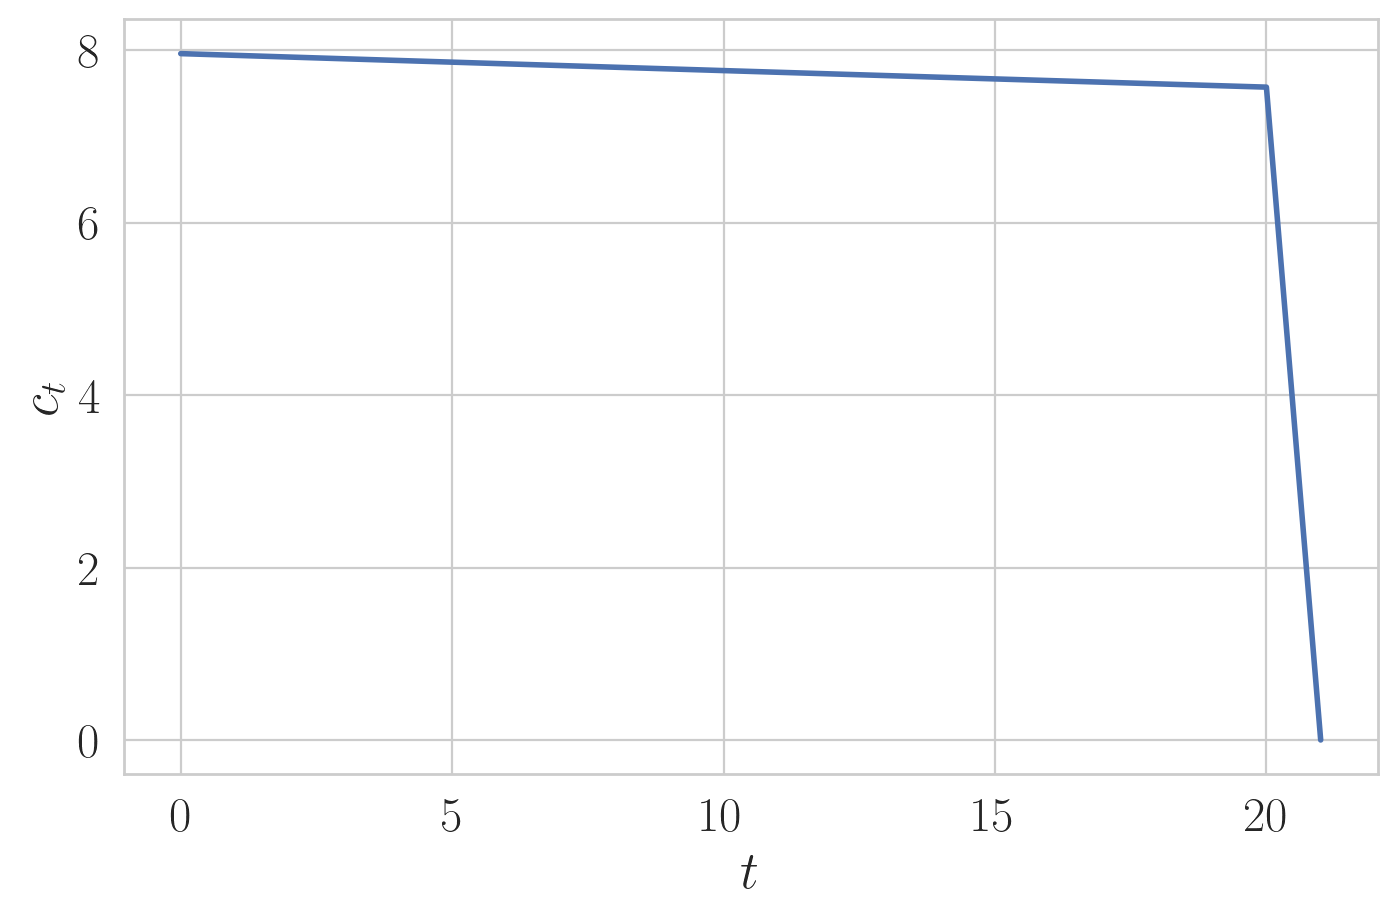
\includegraphics[width=\textwidth]{FH_consumption.png}	
		\caption{Consumption}
	\end{subfigure}
	\begin{subfigure}[b]{0.45\textwidth}
		\centering
		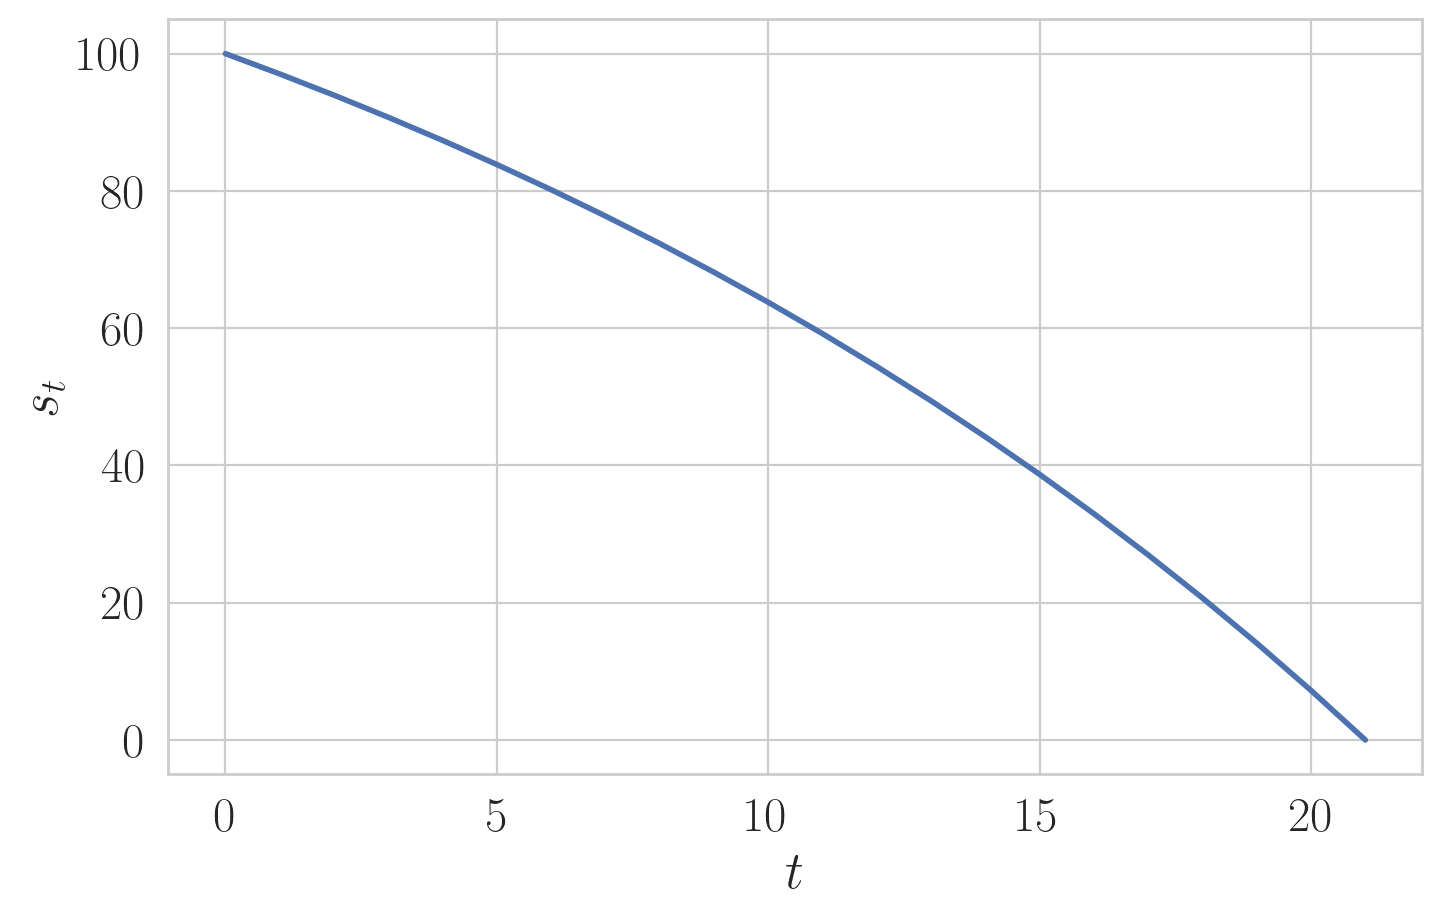
\includegraphics[width=\textwidth]{FH_savings.png}
		\caption{Savings}
	\end{subfigure}
\caption*{$T=20$, $\beta=0.95$, $r=0.05$, $s_{0}=100$.}
\end{figure}

\end{frame}

%%%%%%%%%%%%%%%%%%%%%%%%%%%%%%%%%%%%%%%%%%%%%%%%%%%%%
\begin{frame}{Infinite Horizon Consumption-Savings Problem}

What happens if we allow the agent to be infinitely lived and push $T \to \infty$.


\begin{align*}
\max \quad & \sum_{t=0}^{\infty} \beta^{t} U(c_{t})\\
\text{s.t.} \quad & c_{t} + s_{t+1} = y_{t} + (1+r)s_{t} \quad t = 0,\dots, T\\
& \lim_{t\to\infty} \beta^{t} U^{\prime}(c_{t}) s_{T+1} = 0\\
&s_{0}
\end{align*}

Notice that our previous boundary condition now looks like $\lim_{t\to\infty} \beta^{t} U^{\prime}(c_{t}) s_{T+1} = 0$. This is called the \bc{transversality condition}.
\end{frame}

%%%%%%%%%%%%%%%%%%%%%%%%%%%%%%%%%%%%%%%%%%%%%%%%%%%%%
\begin{frame}{Infinite Horizon Consumption-Savings Problem}

Our Lagrangian is:

\[\mathcal{L} = \sum_{t=0}^{T}\left \{ \beta^{t}U(c_{t}) + \lambda_{t}[y_{t} + (1+r)s_{t} - c_{t} - s_{t+1}] \right\}\]
\medskip

With optimality conditions:

\begin{align*}
&c_{t}:&      \beta^{t} U^{\prime}(c_{t}) - \lambda_{t} = 0  &  &\forall t\\
&s_{t+1}:&  -\lambda_{t} + (1+r)\lambda_{t+1} = 0         && \forall t\\
&\lambda_{t}:& c_{t} + s_{t+1} = y_{t} + (1+r)s_{t} && \forall t
\end{align*}
\medskip

That's a little bit nicer!
\end{frame}

%%%%%%%%%%%%%%%%%%%%%%%%%%%%%%%%%%%%%%%%%%%%%%%%%%%%%
\begin{frame}{Infinite Horizon Consumption-Savings Problem}

The solution looks the same as before, but now the constants come out a little cleaner. After some algebra we get:

\[ a_{1} = s_{0} \qquad a_{2}= 0\]

\begin{figure}
	\begin{subfigure}[b]{0.45\textwidth}
		\centering
		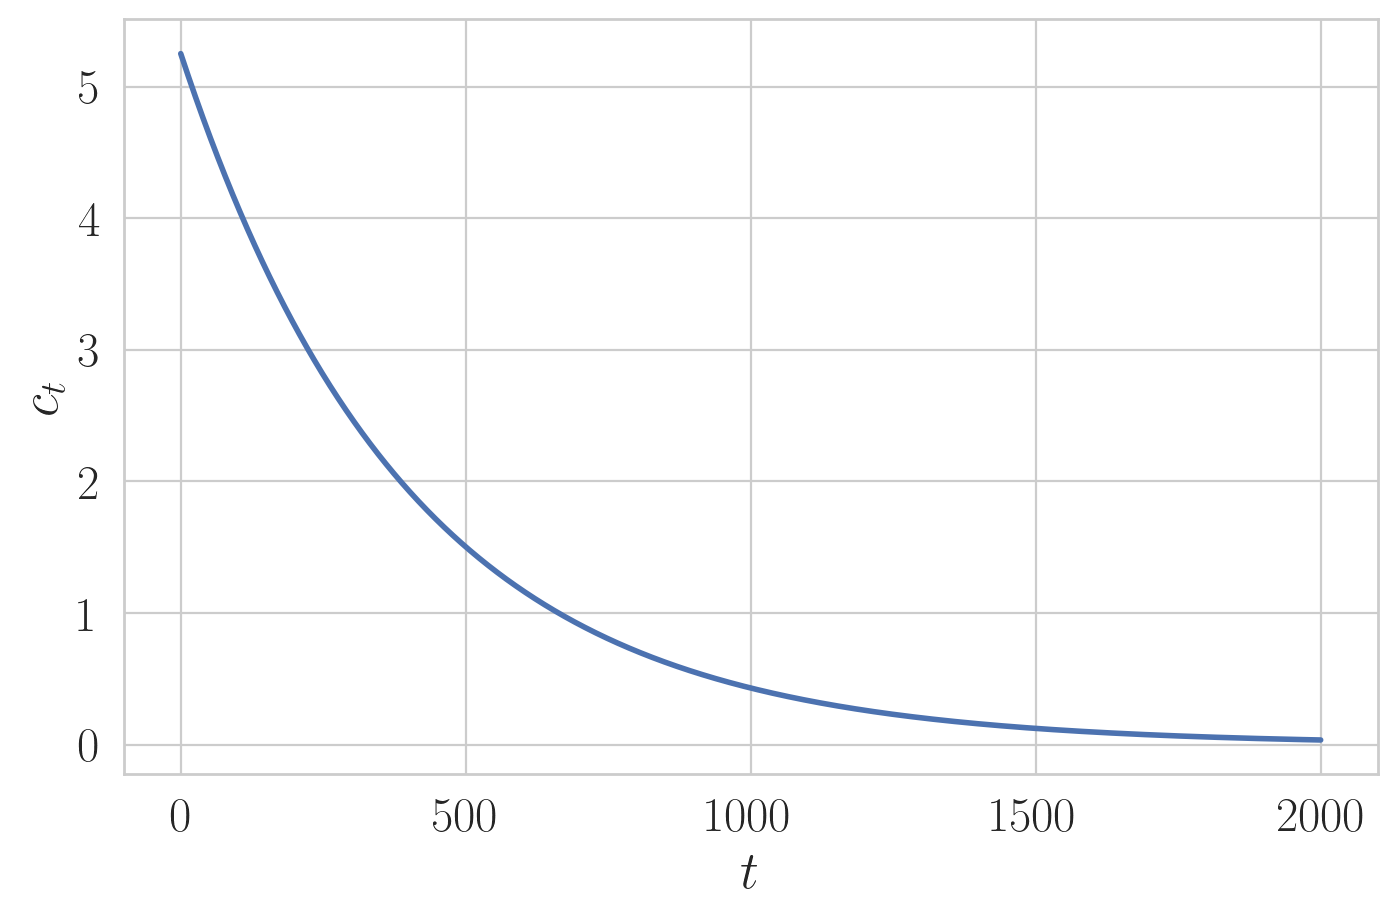
\includegraphics[width=\textwidth]{IH_consumption.png}	
		\caption{Consumption}
	\end{subfigure}
	\begin{subfigure}[b]{0.45\textwidth}
		\centering
		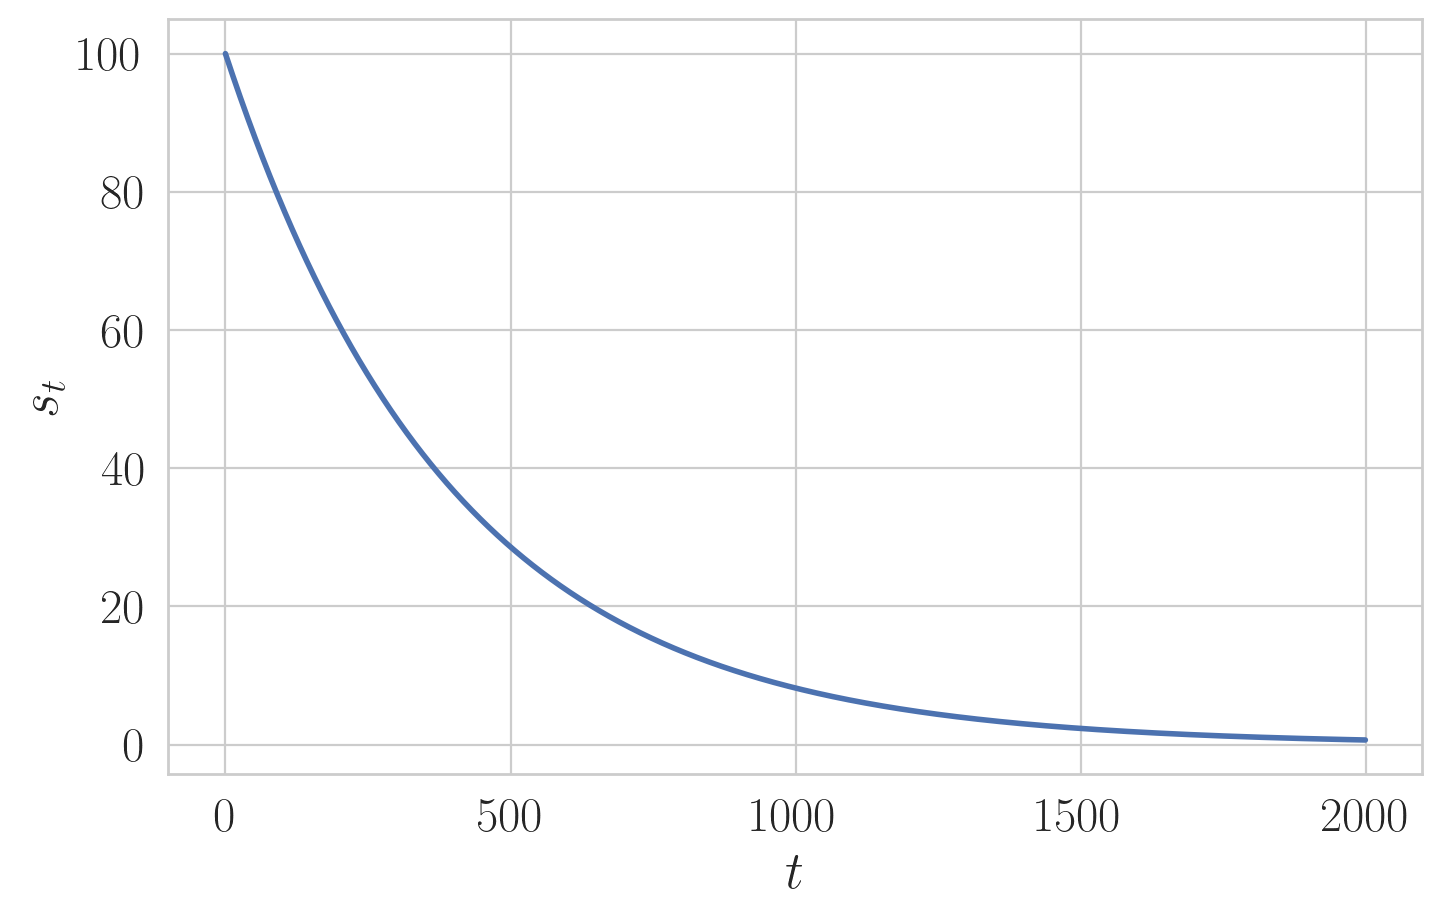
\includegraphics[width=\textwidth]{IH_savings.png}
		\caption{Savings}
	\end{subfigure}
\caption*{$\beta=0.95$, $r=0.05$, $s_{0}=100$}
\end{figure}

\end{frame}

%%%%%%%%%%%%%%%%%%%%%%%%%%%%%%%%%%%%%%%%%%%%%%%%%%%%%
\begin{frame}{Ramsey Growth Model}
There is an infinitely lived agent with logarithmic utility in consumption and discount factor $\beta\in(0, 1)$. This agent begins their life with a stock of capital, $k_{0}$. Each period, the agent uses their capital stock to produce output according to the production technology $F(k_{t}) = Ak_{t}^{\alpha}$, $0 < \alpha < 1$. \medskip

The production process causes capital to depreciate at rate $\delta$. After production, the agent chooses how to allocate output and the remaining capital between consumption in the present period and capital to take into the next period.

\begin{exercise}
	\begin{enumerate}[a)]
	\item Set up the problem and solve for optimality conditions.
	\item Determine if the system admits a steady state.
	\item Log-linearize the system around the steady state.
	\item Characterize the system of first order difference equations.
	
	\end{enumerate}
\end{exercise}
\end{frame}

%%%%%%%%%%%%%%%%%%%%%%%%%%%%%%%%%%%%%%%%%%%%%%%%%%%%%
\begin{frame}{Ramsey Growth Model}
\begin{figure}
	\centering
	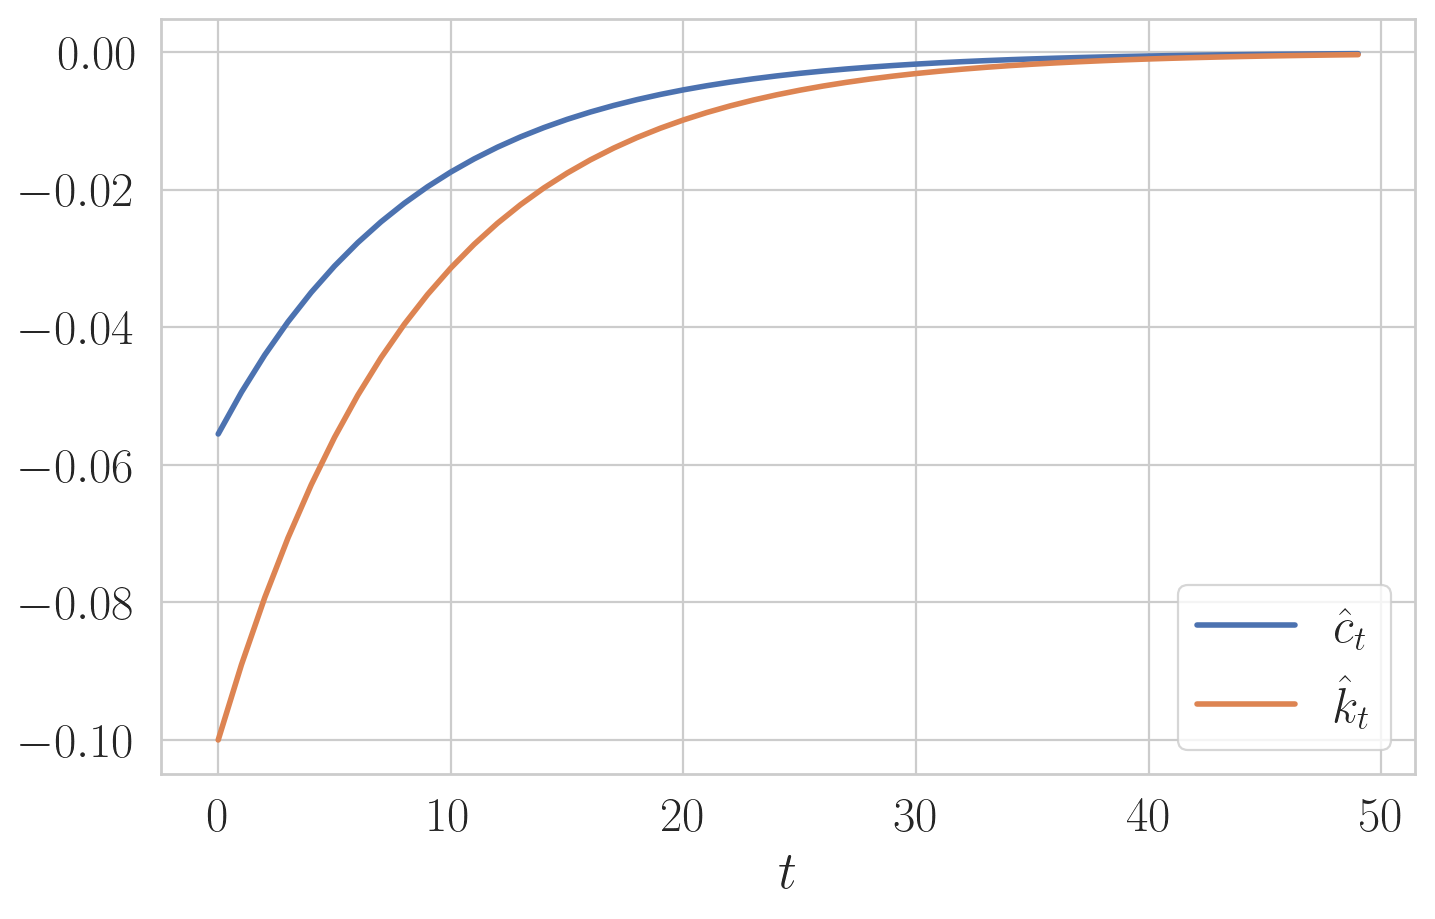
\includegraphics[width=0.75\textwidth]{Ramsey.png}
	\caption{Ramsey model with $\alpha=0.3$, $\beta = 0.95$, $\delta=0.05$, $A=1$, $k_{0}=-0.1$}
\end{figure}
\end{frame}

\begin{frame}{Learning Outcomes}
\bc{You should be able to:}

\begin{enumerate}
	\item Solve unconstrained optimization problems and verify second order conditions.
	\item Set up the Lagrangian and solve.
	\item Log-linearize the optimality conditions around a steady state.
\end{enumerate}
\end{frame}

\end{document}	